\documentclass{jsarticle}

\usepackage{amsmath,amssymb,bm}
\usepackage{graphicx}
\usepackage{ascmac}
\everymath{\displaystyle}
\include{preamble}

\title{有効制約法}

\begin{document}
\maketitle

\section{凸2次計画問題}

2次計画問題とは,
線形不等式$\boldsymbol{A}\boldsymbol{x}\geq\boldsymbol{b}$を満たし,
かつ2次関数$z=\frac{1}{2}\boldsymbol{x}^{\mathrm{T}}\boldsymbol{Q}\boldsymbol{x}+\boldsymbol{c}^{\mathrm{T}}\boldsymbol{x}$の値を最小化する
$\boldsymbol{x}=\boldsymbol{x}^{*}$を求める問題です.
\begin{align*}
\boldsymbol{x}^{*}=\mathop{\mathrm{arg~min}}_{\boldsymbol{x}}\left\{
\left.
z=\frac{1}{2}\boldsymbol{x}^{\mathrm{T}}\boldsymbol{Q}\boldsymbol{x}+\boldsymbol{c}^{\mathrm{T}}\boldsymbol{x}
\right|
\boldsymbol{A}\boldsymbol{x}\geq\boldsymbol{b}
\right\}
\end{align*}
ただし,
$\boldsymbol{Q}$は対称な正方行列であることが仮定されます
($\boldsymbol{Q}$が対称で無い場合,
$\frac{1}{2}\left(\boldsymbol{Q}+\boldsymbol{Q}^{\mathrm{T}}\right)$をあらためて
$\boldsymbol{Q}$とおけば良いです).
$\boldsymbol{x}$は{\bf 設計変数},
$\boldsymbol{x}^{*}$は{\bf 最適解},
$z$は{\bf 目的関数}(あるいは{\bf 評価関数},{\bf 損失関数})などと呼ばれます.
多くの場合,$\boldsymbol{Q}$は正定値行列であると仮定されます.
この時は特に{\bf 凸2次計画問題}と呼ばれます.
$\boldsymbol{Q}$が正定値行列でない場合は一般的に解の存在が保証されず,
難度の高い問題となります.
%本記事では凸2次計画問題のみ扱います.
%その解法は幾つか知られていますが,
凸2次計画問題の解法は幾つか知られていますが,
{\bf 有効制約法}(Active Set Method)はシンプルで,
かつ問題の規模がさほど大きくなければ十分実用的な方法です.
本記事では,実装まで意識してその内容を説明します.


「有効制約法」はオーソライズされた用語ですが,個人的にはこれはあまり良い訳と思えません.
計算の過程で制約(不等式制約)は常に有効です.
この点,混乱を招くからです.
アルゴリズムからは,``Active Set''は「有効化された{\bf 等式の}集合」と解釈すべきですが,
残念ながらこれをずばりと表現する良い単語に筆者は思い至りません.
「Active Set法」と呼ぶのがいちばん良いような気がします.
が,筆者一人がそのようなことを呟いてもしょうがないので,
本記事ではオーソライズされた用語を用います(我ながら弱気です).



\section{KKT条件}

有効制約法のアルゴリズムを考える上では,
{\bf KKT(Karush-Kuhn-Tucker)条件}の理解が欠かせません.
これを説明します.
以下,
$\boldsymbol{x}$の次数が$n$であるとして,
次の非線形計画問題を考えましょう.
\begin{align*}
\boldsymbol{x}^{*}=\mathop{\mathrm{arg~min}}_{\boldsymbol{x}}\left\{
\left.
z=E(\boldsymbol{x})
\right|
g(\boldsymbol{x})\geq 0
\right\}
\end{align*}
ただし,評価関数$z=E(\boldsymbol{x})$は下に凸で,
ただ一つの極小点$\bar{\boldsymbol{x}}$を持つものとします.
また,$E(\boldsymbol{x})$も$g(\boldsymbol{x})$も
任意の$\boldsymbol{x}$について微分可能であると仮定します.
%$\bar{\boldsymbol{x}}$は次の条件を満たします.
%\begin{align*}
%\left(\frac{\partial E}{\partial\boldsymbol{x}}\right)^{\mathrm{T}}(\bar{\boldsymbol{x}})=\boldsymbol{0}
%\end{align*}

いま,$g(\boldsymbol{x})=0$で表される超曲線と接する
$z=E(\boldsymbol{x})$の等高線がただ一つだけあるとします
(この仮定は割と厳しいものですが,凸2次計画問題においては常に真となります).
このとき次が言えます(下図参照).
\begin{itemize}
\item{
$g(\bar{\boldsymbol{x}})\geq 0$ならば,
$\bar{\boldsymbol{x}}$が最適解$\boldsymbol{x}^{*}$
}
\item{
$g(\bar{\boldsymbol{x}})<0$ならば,
$g(\boldsymbol{x})=0$に接する$z=E(\boldsymbol{x})$の等高線の接点が最適解$\boldsymbol{x}^{*}$
}
\end{itemize}

\begin{figure}[h]
\begin{center}
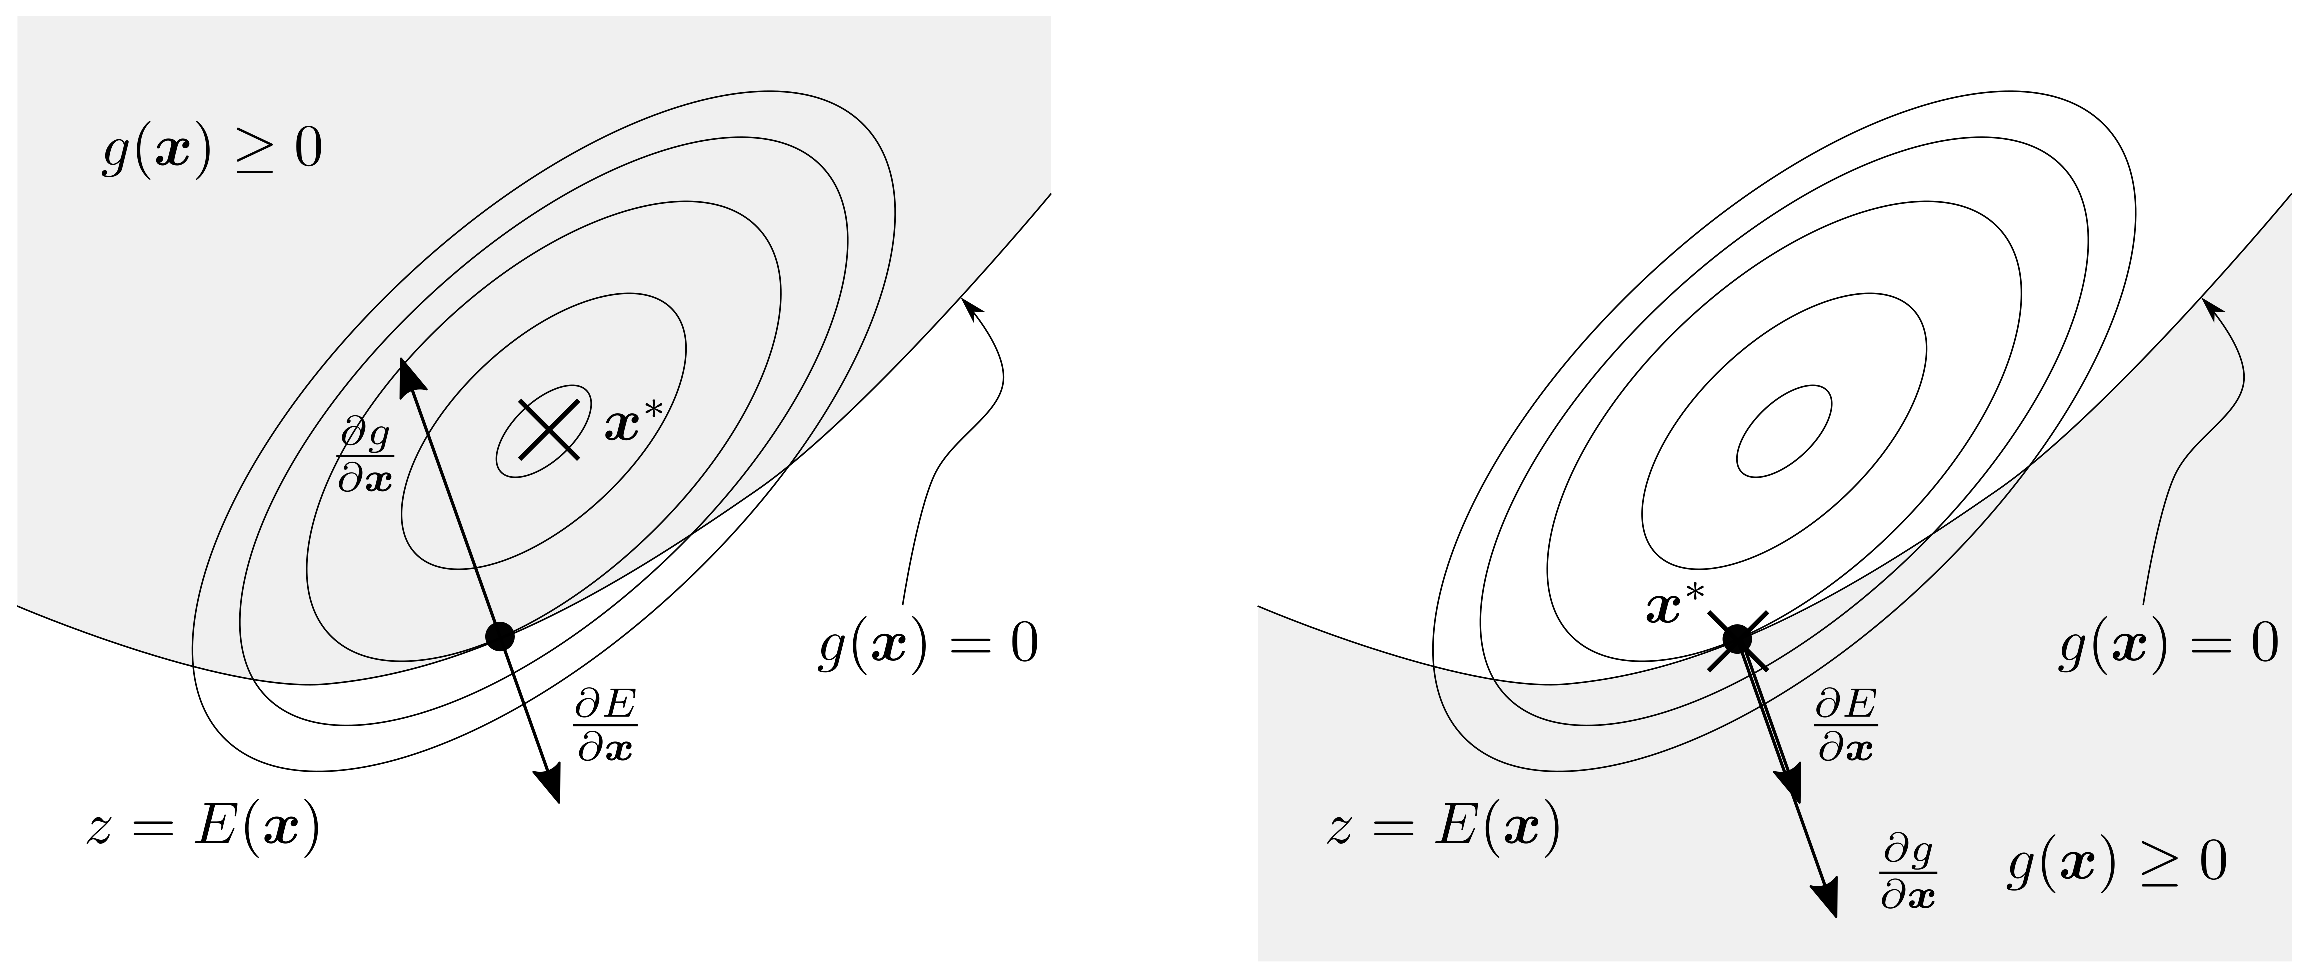
\includegraphics[width=.8\textwidth]{fig/Kuhn-Tucker.eps}
\end{center}
\end{figure}

ここで,
$g(\boldsymbol{x})=0$と$z=E(\boldsymbol{x})$の等高線との接点
$\boldsymbol{x}$から等高線に沿って無限小量$\mathrm{d}\boldsymbol{x}$動いた点を考えると,
\begin{align*}
E(\boldsymbol{x}+\mathrm{d}\boldsymbol{x})=E(\boldsymbol{x})
\end{align*}
ですので
\begin{align*}
E(\boldsymbol{x}+\mathrm{d}\boldsymbol{x})-E(\boldsymbol{x})
\simeq\left(\frac{\partial E}{\partial\boldsymbol{x}}\right)^{\mathrm{T}}\mathrm{d}\boldsymbol{x}
=0
\end{align*}
となります.
$\mathrm{d}\boldsymbol{x}$は等高線の接ベクトルですから,
$\left(\frac{\partial E}{\partial\boldsymbol{x}}\right)^{\mathrm{T}}$は
$\boldsymbol{x}$における$E(\boldsymbol{x})$の等高線に直交するベクトル,
すなわち法線ベクトルとなることが分かります.
同じ点から,
今度は$\left(\frac{\partial E}{\partial\boldsymbol{x}}\right)^{\mathrm{T}}$の方向に無限小量
$\varepsilon\left(\frac{\partial E}{\partial\boldsymbol{x}}\right)^{\mathrm{T}}$
(ただし$\varepsilon>0$とします)動いた点を考えると,
\begin{align*}
E\left(\boldsymbol{x}+\varepsilon\left(\frac{\partial E}{\partial\boldsymbol{x}}\right)^{\mathrm{T}}\right)
-E(\boldsymbol{x})
\simeq\varepsilon\left\|\left(\frac{\partial E}{\partial\boldsymbol{x}}\right)^{\mathrm{T}}\right\|^{2}
\geq 0
\end{align*}
であるので,
$\left(\frac{\partial E}{\partial\boldsymbol{x}}\right)^{\mathrm{T}}$は
$E(\boldsymbol{x})$が増加する方向を向いていることも分かります.
全く同様の考察により,
$\left(\frac{\partial g}{\partial\boldsymbol{x}}\right)^{\mathrm{T}}$は
$g(\boldsymbol{x})=0$の$\boldsymbol{x}$における法線ベクトルとなり,
しかも$g(\boldsymbol{x})$が増加する方向を向いていると分かります.

$z=E(\boldsymbol{x})$の等高線が$g(\boldsymbol{x})=0$に接するということは,
$g(\boldsymbol{x})=0$上のある点において両者の法線が一致する,
すなわち
\begin{align*}
\left(\frac{\partial E}{\partial\boldsymbol{x}}\right)^{\mathrm{T}}-\lambda\left(\frac{\partial g}{\partial\boldsymbol{x}}\right)^{\mathrm{T}}=\boldsymbol{0}
\end{align*}
を満たす定数$\lambda$が存在するということになります.
特に
$\left(\frac{\partial E}{\partial\boldsymbol{x}}\right)^{\mathrm{T}}$と$\left(\frac{\partial g}{\partial\boldsymbol{x}}\right)^{\mathrm{T}}$が同じ方向を向いている
($\bar{\boldsymbol{x}}$が領域$g(\boldsymbol{x})>0$にないケース)ならば,
$\lambda$は正でなければなりません.
また,
$\bar{\boldsymbol{x}}$は
$\left(\frac{\partial E}{\partial\boldsymbol{x}}(\bar{\boldsymbol{x}})\right)^{\mathrm{T}}=\boldsymbol{0}$を満たします.
このことから,
最適解$\boldsymbol{x}^{*}$が満たす条件は
\begin{align*}
g(\boldsymbol{x}^{*})>0 \quad\mbox{かつ}\quad
\left(\frac{\partial E}{\partial\boldsymbol{x}}(\boldsymbol{x}^{*})\right)^{\mathrm{T}}=\boldsymbol{0}
\end{align*}
または
\begin{align*}
g(\boldsymbol{x}^{*})=0 \quad\mbox{かつ}\quad
\left(\frac{\partial E}{\partial\boldsymbol{x}}(\boldsymbol{x}^{*})\right)^{\mathrm{T}}
-\lambda
\left(\frac{\partial g}{\partial\boldsymbol{x}}(\boldsymbol{x}^{*})\right)^{\mathrm{T}}
=\boldsymbol{0}
\mbox{を満たす$\lambda>0$が存在する}
\end{align*}
となります.
これらは
\begin{align*}
\left(\frac{\partial E}{\partial\boldsymbol{x}}(\boldsymbol{x}^{*})\right)^{\mathrm{T}}
-\lambda
\left(\frac{\partial g}{\partial\boldsymbol{x}}(\boldsymbol{x}^{*})\right)^{\mathrm{T}}
=\boldsymbol{0}
\\
g(\boldsymbol{x}^{*})>0 \quad\mbox{かつ}\quad \lambda=0,
\qquad\mbox{または}\qquad
g(\boldsymbol{x}^{*})=0 \quad\mbox{かつ}\quad \lambda>0
\end{align*}
のように巧妙にまとめられます.

制約条件が複数本($m$本とします)ある問題
\begin{align*}
\boldsymbol{x}^{*}=\mathop{\mathrm{arg~min}}_{\boldsymbol{x}}\left\{
\left.
z=E(\boldsymbol{x})
\right|
g_{1}(\boldsymbol{x})\geq 0, \cdots, g_{m}(\boldsymbol{x})\geq 0
\right\}
\end{align*}
の場合も考え方は同じで,
\begin{align*}
\boldsymbol{g}(\boldsymbol{x})\overset{\mathrm{def}}{=}\left[\begin{array}{c}
g_{1}(\boldsymbol{x}) \\
g_{2}(\boldsymbol{x}) \\
\vdots \\
g_{m}(\boldsymbol{x}) \\
\end{array}\right]
,\qquad
\boldsymbol{\lambda}\overset{\mathrm{def}}{=}\left[\begin{array}{c}
\lambda_{1} \\
\lambda_{2} \\
\vdots \\
\lambda_{m} \\
\end{array}\right]
\end{align*}
とおくと,
最適解$\boldsymbol{x}^{*}$は
\begin{align*}
\left(\frac{\partial E}{\partial\boldsymbol{x}}(\boldsymbol{x}^{*})\right)^{\mathrm{T}}
-
\left(\frac{\partial\boldsymbol{g}}{\partial\boldsymbol{x}}(\boldsymbol{x}^{*})\right)^{\mathrm{T}}
\boldsymbol{\lambda}
=\boldsymbol{0}
\end{align*}
かつ全ての$i\in\mathcal{I}=\left\{1,\cdots,m\right\}$について
\begin{align*}
g_{i}(\boldsymbol{x}^{*})>0 \quad\mbox{かつ}\quad \lambda_{i}=0,
\qquad\mbox{または}\qquad
g_{i}(\boldsymbol{x}^{*})=0 \quad\mbox{かつ}\quad \lambda_{i}>0
\end{align*}
を満たします.
これがKKT条件です.

分かりやすいように,
$n=2$,
$z=E(\boldsymbol{x})$を同心円状の等高線を持つ関数,
$\boldsymbol{g}(\boldsymbol{x})=\boldsymbol{0}$を2本の直線として
KKT条件を図解したものを下に示します.
\begin{figure}[h]
\begin{center}
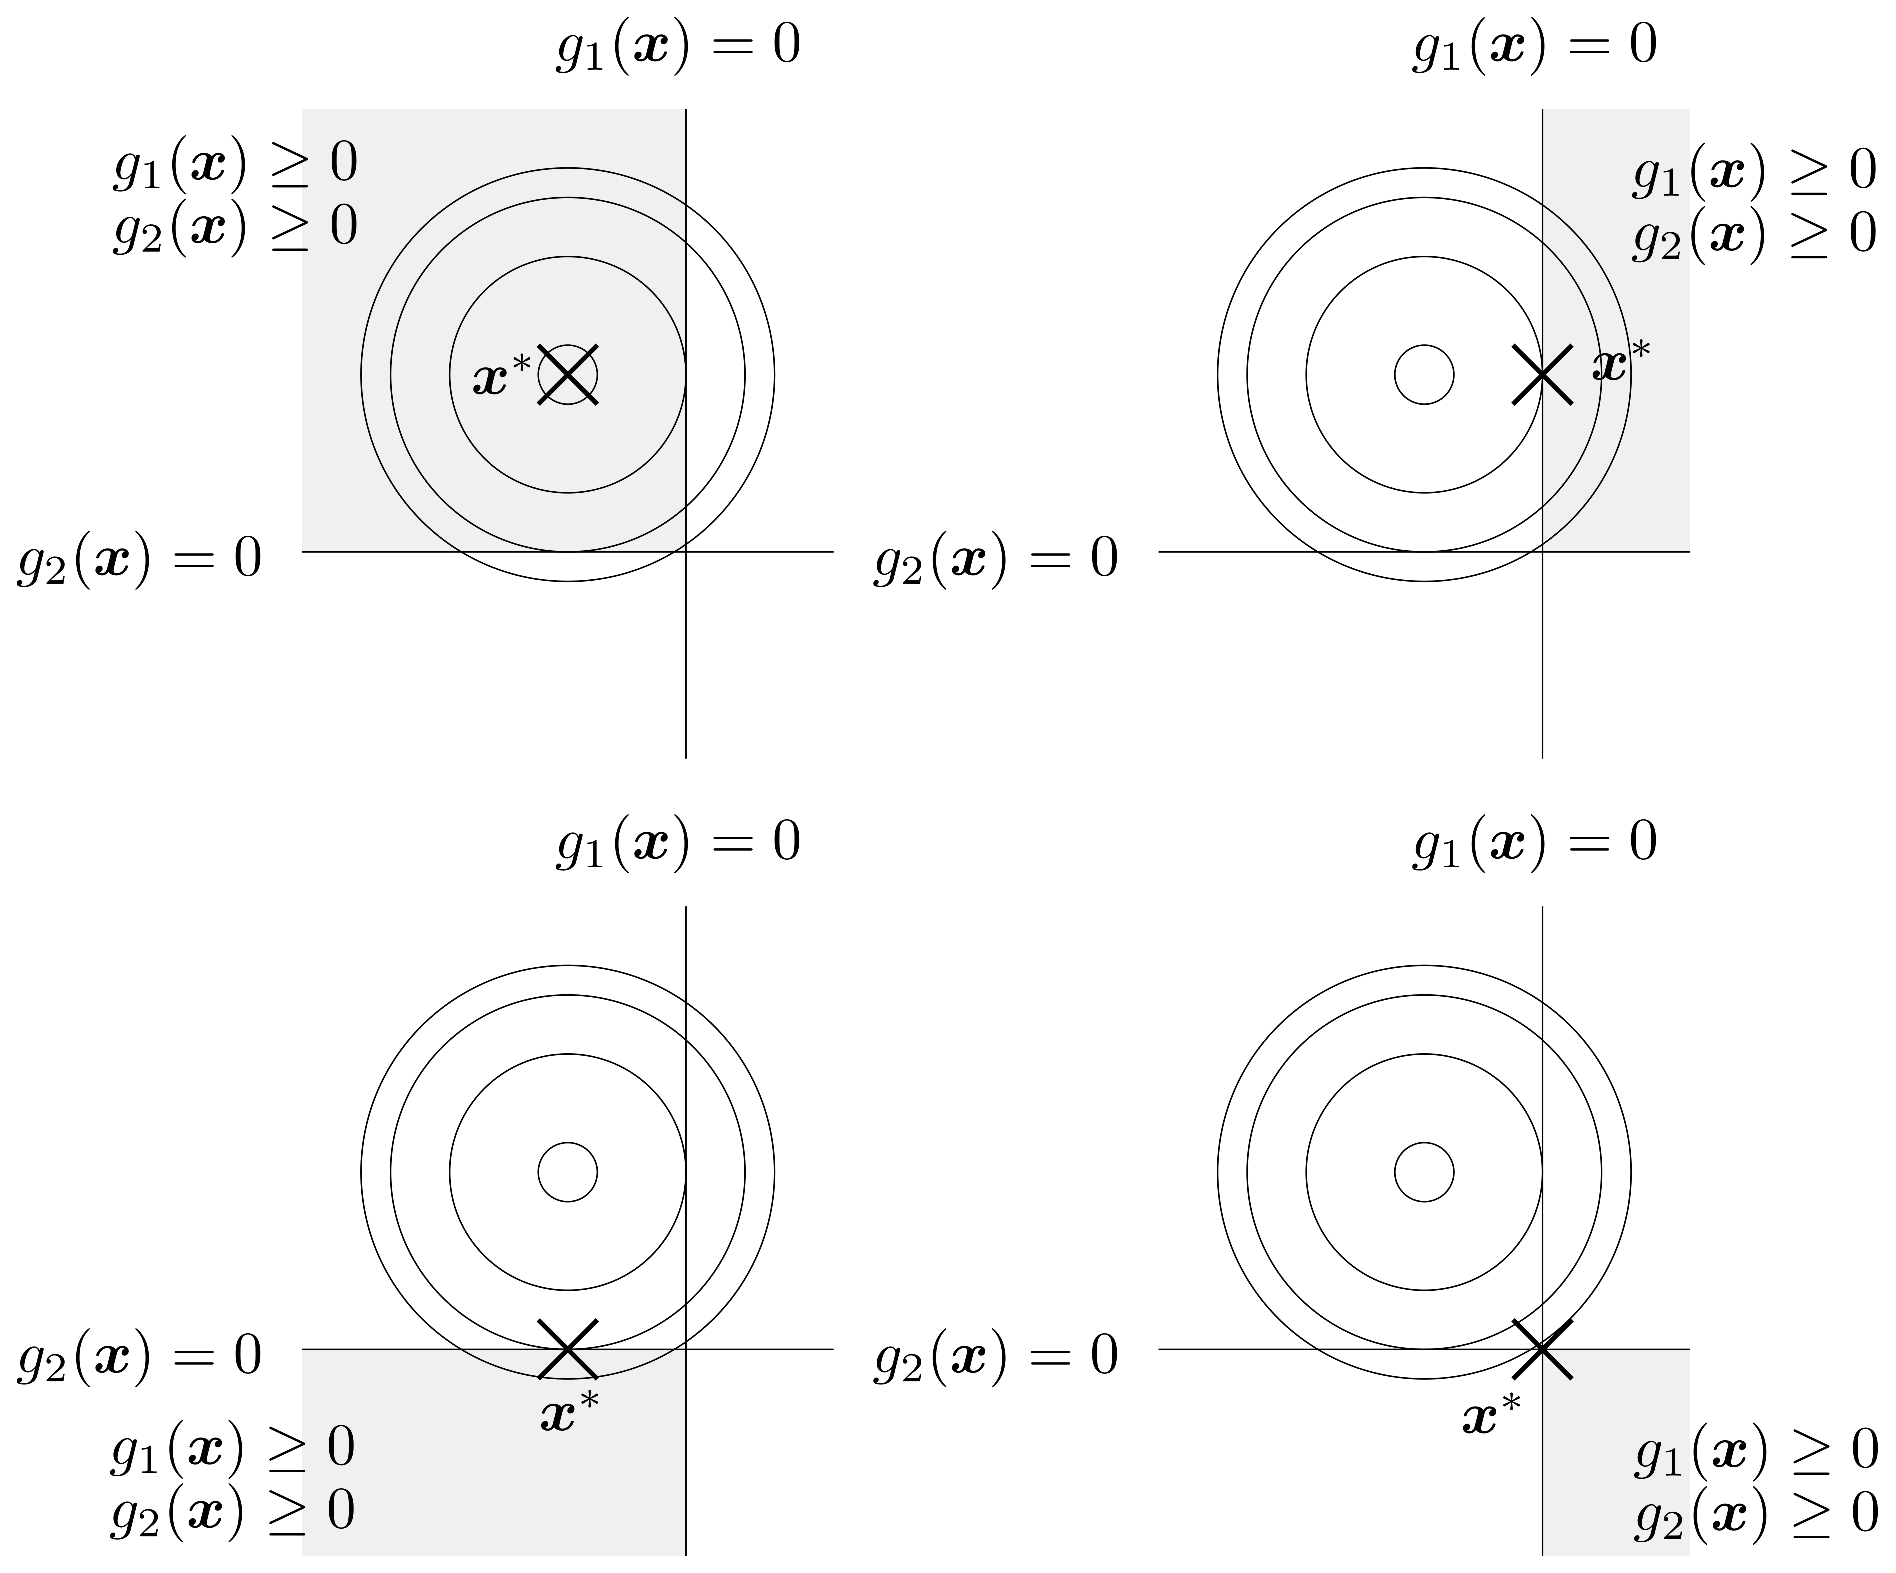
\includegraphics[width=.5\textwidth]{fig/Kuhn-Tucker-2.eps}
\end{center}
\end{figure}


\section{有効制約法のアルゴリズム}

\subsection{考え方と流れ}

前節で述べたKKT条件を踏まえて,
元の凸2次計画問題を考えましょう.
$\boldsymbol{A}$の$i$行目ベクトルを$\boldsymbol{a}_{i}^{\mathrm{T}}$,
$\boldsymbol{b}$の$i$番目成分を$b_{i}$とそれぞれおくと,
$E(\boldsymbol{x})=\frac{1}{2}\boldsymbol{x}^{\mathrm{T}}\boldsymbol{Q}\boldsymbol{x}+\boldsymbol{c}^{\mathrm{T}}\boldsymbol{x}$,
$g_{i}(\boldsymbol{x})=\boldsymbol{a}_{i}^{\mathrm{T}}\boldsymbol{x}-b_{i}$($i\in\mathcal{I}=\left\{1,\cdots,m\right\}$)です.
今,最適解$\boldsymbol{x}^{*}$が,
幾つかの$i\in\mathcal{I}^{*}(\subseteq\mathcal{I})$に対して
$\boldsymbol{a}_{i}^{\mathrm{T}}\boldsymbol{x}^{*}=b_{i}$を満たし,
残りの$i\in\bar{\mathcal{I}}^{*}\overset{\mathrm{def}}{=}\mathcal{I}\setminus\mathcal{I}^{*}$に対しては,
$\boldsymbol{a}_{i}^{\mathrm{T}}\boldsymbol{x}^{*}>b_{i}$を満たすか,
または$\boldsymbol{a}_{i}^{\mathrm{T}}\boldsymbol{x}^{*}=b_{i}$が
等式群$\left\{\boldsymbol{a}_{i}^{\mathrm{T}}\boldsymbol{x}^{*}=b_{i}\left|\forall i\in\mathcal{I}^{*}\right.\right\}$に
従属であるとします.
前者を$\boldsymbol{A}^{*}\boldsymbol{x}^{*}=\boldsymbol{b}^{*}$,
後者を$\bar{\boldsymbol{A}}^{*}\boldsymbol{x}^{*}\geq\bar{\boldsymbol{b}}^{*}$,
さらに前者に対応する$\lambda_{i}$($\forall i\in\mathcal{I}^{*}$)を$\boldsymbol{\lambda}^{*}$と
それぞれまとめれば,
KKT条件より次が成り立ちます.
\begin{align*}
\boldsymbol{Q}\boldsymbol{x}^{*}+\boldsymbol{c}
-\boldsymbol{A}^{*\mathrm{T}}\boldsymbol{\lambda}^{*}
=\boldsymbol{0}
\\
\boldsymbol{A}^{*}\boldsymbol{x}^{*}-\boldsymbol{b}^{*}=\boldsymbol{0}
\\
\boldsymbol{\lambda}^{*}>\boldsymbol{0}
\\
\bar{\boldsymbol{A}}^{*}\boldsymbol{x}^{*}-\bar{\boldsymbol{b}}^{*}\geq\boldsymbol{0}
\end{align*}
もし$\boldsymbol{A}^{*}$と$\boldsymbol{b}^{*}$があらかじめ分かっているならば,
最初の二つの方程式を連立して解くことで
$\boldsymbol{x}^{*}$および$\boldsymbol{\lambda}^{*}$が次のように得られます.
\begin{align*}
\boldsymbol{\lambda}^{*}
=
\left(\boldsymbol{A}^{*}\boldsymbol{Q}^{-1}\boldsymbol{A}^{*\mathrm{T}}\right)^{-1}
\left(
\boldsymbol{A}^{*}\boldsymbol{Q}^{-1}\boldsymbol{c}
+
\boldsymbol{b}^{*}
\right)
\\
\boldsymbol{x}^{*}
=
\boldsymbol{Q}^{-1}
\left(
\boldsymbol{A}^{*\mathrm{T}}\boldsymbol{\lambda}^{*}-\boldsymbol{c}
\right)
\end{align*}
$\boldsymbol{A}^{*}\boldsymbol{x}^{*}=\boldsymbol{b}^{*}$は独立な等式しか含まないので,
$\boldsymbol{A}^{*}$が行フルランクとなることにご注意下さい.
このとき,残りの二つの不等式も成り立つはずです.
したがって,
\begin{screen}
\begin{enumerate}
\item{$\mathcal{I}$から適当に幾つかの要素を選んで$\mathcal{I}^{*}$の候補$\mathcal{I}^{\prime}$を作り,
それ以外の要素を$\bar{\mathcal{I}}^{\prime}$とまとめる.}
\item{$\boldsymbol{a}_{i}^{\mathrm{T}}$,$b_{i}$($\forall i\in\mathcal{I}^{\prime}$)をまとめて
それぞれ$\boldsymbol{A}^{\prime}$,$\boldsymbol{b}^{\prime}$とおく.}
\item{
$\boldsymbol{x}^{\prime}$および$\boldsymbol{\lambda}^{\prime}$を
\begin{align*}
\boldsymbol{\lambda}^{\prime}
=
\left(\boldsymbol{A}^{\prime}\boldsymbol{Q}^{-1}\boldsymbol{A}^{\prime\mathrm{T}}\right)^{-1}
\left(
\boldsymbol{A}^{\prime}\boldsymbol{Q}^{-1}\boldsymbol{c}
+
\boldsymbol{b}^{\prime}
\right)
\\
\boldsymbol{x}^{\prime}
=
\boldsymbol{Q}^{-1}
\left(
\boldsymbol{A}^{\prime\mathrm{T}}\boldsymbol{\lambda}^{\prime}-\boldsymbol{c}
\right)
\end{align*}
と求める.}
\item{
$\boldsymbol{a}_{i}^{\mathrm{T}}\boldsymbol{x}^{\prime}>b_{i}$($\forall i\in\bar{\mathcal{I}}^{\prime}$)および
$\lambda_{i}>0$($\forall i\in\mathcal{I}^{\prime}$)が満たされているならば,
$\boldsymbol{x}^{*}=\boldsymbol{x}^{\prime}$として終了.}
\item{$\mathcal{I}^{\prime}$を適当に作り変えて2に戻る.}
\end{enumerate}
\end{screen}
という方法を思いつきます.
等式群$\left\{\boldsymbol{a}_{i}^{\mathrm{T}}\boldsymbol{x}^{*}=b_{i}\left|\forall i\in\mathcal{I}^{\prime}\right.\right\}$
のみを{\bf 有効制約}として抽出し,
等式制約付き最適化問題として問いた後に,
残り不等式制約が満たされているかチェックする,ということです.

アルゴリズムとして採用するには「適当」では困りますから,
システマティックに$\mathcal{I}^{\prime}$を修正していく方法が必要です.
$\mathcal{I}$から$\mathcal{I}^{\prime}$を作る組み合わせは$\sum_{j=0}^{m}{}_{m}C_{j}$通りあるので,
網羅的に調べるのは効率が良くありません.
そこで,上記を次のように修正します.
\begin{screen}
\begin{enumerate}
\item{
$\boldsymbol{a}_{i}^{\mathrm{T}}\boldsymbol{x}_{0}=b_{i}$($\forall i\in\mathcal{I}^{\prime}\subseteq\mathcal{I}$)かつ
$\boldsymbol{a}_{i}^{\mathrm{T}}\boldsymbol{x}_{0}\geq b_{i}$($\forall i\in\bar{\mathcal{I}}^{\prime}=\mathcal{I}\setminus\mathcal{I}^{\prime}$)を満たす$\mathcal{I}^{\prime}$,$\bar{\mathcal{I}}^{\prime}$の組と$\boldsymbol{x}_{0}$を一つ見つける.({\bf 初期有効制約の発見})}
\item{
$\boldsymbol{a}_{i}^{\mathrm{T}}$,$b_{i}$($\forall i\in\mathcal{I}^{\prime}$)をまとめて
それぞれ$\boldsymbol{A}^{\prime}$,$\boldsymbol{b}^{\prime}$とおく.
}
\item{$\boldsymbol{x}^{\prime}$および$\boldsymbol{\lambda}^{\prime}$を次式より求める.
\begin{align*}
\boldsymbol{\lambda}^{\prime}
=
\left(\boldsymbol{A}^{\prime}\boldsymbol{Q}^{-1}\boldsymbol{A}^{\prime\mathrm{T}}\right)^{-1}
\left(
\boldsymbol{A}^{\prime}\boldsymbol{Q}^{-1}\boldsymbol{c}
+
\boldsymbol{b}^{\prime}
\right)
\\
\boldsymbol{x}^{\prime}
=
\boldsymbol{Q}^{-1}
\left(
\boldsymbol{A}^{\prime\mathrm{T}}\boldsymbol{\lambda}^{\prime}-\boldsymbol{c}
\right)
\end{align*}
}
\item{
$\boldsymbol{a}_{i}^{\mathrm{T}}\boldsymbol{x}^{\prime}<b_{i}$($i\in\bar{\mathcal{I}}^{\prime}$)となる
$i$が一つでもあれば,
そのうち最も$\boldsymbol{x}_{0}$に近いものを$\bar{\mathcal{I}}^{\prime}$から$\mathcal{I}^{\prime}$に移し,
$\boldsymbol{x}_{0}$を更新して3に戻る.
({\bf 有効制約の追加})}
\item{$\lambda_{i}<0$($i\in\mathcal{I}^{\prime}$)となる一つの$i$を
$\mathcal{I}^{\prime}$から除外し$\bar{\mathcal{I}}^{\prime}$に移す.
({\bf 有効制約の除外})
$\lambda_{i}<0$($i\in\mathcal{I}^{\prime}$)となる$i$が一つもなければ,
$\boldsymbol{x}^{*}=\boldsymbol{x}^{\prime}$として終了.}
\item{2に戻る.}
\end{enumerate}
\end{screen}
つまり,
不等式制約条件に不充足があればそれを解消するよう等式制約条件を増やし,
目的関数をさらに減少させる余地があるならば等式制約条件を減らす,
その反復によって有効制約を更新していくということです.
これが有効制約法の基本的な流れです.
拠り所となる$\boldsymbol{x}_{0}$を同時に更新していくのが一つのポイントになります.

太字で書いた3項目の詳細を,次節以降で説明します.

\subsection{初期有効制約の発見}

「$\boldsymbol{a}_{i}^{\mathrm{T}}\boldsymbol{x}_{0}=b_{i}$($\forall i\in\mathcal{I}^{\prime}\subseteq\mathcal{I}$)かつ
$\boldsymbol{a}_{i}^{\mathrm{T}}\boldsymbol{x}_{0}\geq b_{i}$($\forall i\in\bar{\mathcal{I}}^{\prime}=\mathcal{I}\setminus\mathcal{I}^{\prime}$)を満たす$\mathcal{I}^{\prime}$,$\bar{\mathcal{I}}^{\prime}$の組と$\boldsymbol{x}_{0}$を一つ見つける」には,
線形計画問題に対する2段階単体法の1段目計算を応用できます.
別記事もご参照下さい.
ここでは要点だけ記します.

線形計画問題とは,ある線形方程式を満たす非負変数の組のうち,ある線形関数の値を最小にするものを求める問題です.
線形不等式は,次のように非負変数を用いた線形方程式に置き換えられます.
\begin{align*}
\boldsymbol{A}\boldsymbol{x}\geq\boldsymbol{b}
\quad\Leftrightarrow\quad
\boldsymbol{A}(\boldsymbol{x}_{+}-\boldsymbol{x}_{-})-\boldsymbol{x}_{\mathrm{S}}=\boldsymbol{b}
,\quad
\boldsymbol{x}_{+}\geq\boldsymbol{0},\quad
\boldsymbol{x}_{-}\geq\boldsymbol{0},\quad
\boldsymbol{x}_{\mathrm{S}}\geq\boldsymbol{0}
\end{align*}
ただし,
$\boldsymbol{x}=\boldsymbol{x}_{+}-\boldsymbol{x}_{-}$
の関係があります.
$\boldsymbol{x}_{\mathrm{S}}$はスラック変数と呼ばれます.
上記は次のようにも書けます.
\begin{align*}
\begin{bmatrix}
\boldsymbol{A} & -\boldsymbol{A} & -\boldsymbol{1}
\end{bmatrix}
\begin{bmatrix}
\boldsymbol{x}_{+} \\ \boldsymbol{x}_{-} \\ \boldsymbol{x}_{\mathrm{S}}
\end{bmatrix}
=
\boldsymbol{b}
,\qquad
\begin{bmatrix}
\boldsymbol{x}_{+} \\ \boldsymbol{x}_{-} \\ \boldsymbol{x}_{\mathrm{S}}
\end{bmatrix}
\geq\boldsymbol{0}
\end{align*}
先に進む前に,
$b_{i}<0$となる全ての$i$について,左辺係数行列の$i$行目および$b_{i}$の符号を反転させ,
上記の等式を次のように書き換えましょう.
\begin{align*}
\begin{bmatrix}
\boldsymbol{A}_{+} & -\boldsymbol{A}_{+} & \boldsymbol{S}
\end{bmatrix}
\begin{bmatrix}
\boldsymbol{x}_{+} \\ \boldsymbol{x}_{-} \\ \boldsymbol{x}_{\mathrm{S}}
\end{bmatrix}
=
\tilde{\boldsymbol{b}}
\end{align*}
$\tilde{\boldsymbol{b}}=\left[\tilde{b}_{1}~\cdots~\tilde{b}_{m}\right]^{\mathrm{T}}$は,
全ての成分が非負であると前提できます.
この下で,次の線形計画問題を考えます.
\begin{align*}
\tilde{\boldsymbol{x}}^{*}=\mathop{\mathrm{arg~min}}_{\tilde{\boldsymbol{x}}}\left\{
\left.
\boldsymbol{l}^{\mathrm{T}}\boldsymbol{x}_{\mathrm{L}}
\right|
\tilde{\boldsymbol{A}}\tilde{\boldsymbol{x}}=\tilde{\boldsymbol{b}}
,\quad
\tilde{\boldsymbol{x}}\geq\boldsymbol{0}
\right\}
\end{align*}
ただし,
\begin{align*}
\tilde{\boldsymbol{A}}\overset{\mathrm{def}}{=}\begin{bmatrix}
\boldsymbol{A}_{+} & -\boldsymbol{A}_{+} & \boldsymbol{S} & \boldsymbol{1}
\end{bmatrix}
,\qquad
\tilde{\boldsymbol{x}}\overset{\mathrm{def}}{=}\begin{bmatrix}
\boldsymbol{x}_{+} \\ \boldsymbol{x}_{-} \\ \boldsymbol{x}_{\mathrm{S}} \\ \boldsymbol{x}_{\mathrm{L}}
\end{bmatrix}
,\qquad
\boldsymbol{l}\overset{\mathrm{def}}{=}\left[1~\cdots~1\right]^{\mathrm{T}}
\end{align*}
とそれぞれおきました.
$\boldsymbol{x}_{\mathrm{L}}$は{\bf 人為変数}と呼ばれます.
$\tilde{\boldsymbol{b}}\geq\boldsymbol{0}$なので,最適解は単体法によって簡単に求まり,
同時に
基底変数のインデックス群$\mathcal{J}_{\mathrm{B}}$(要素数$m$個),
非基底変数のインデックス群$\mathcal{J}_{\mathrm{N}}$(要素数$2n+m$個),
独立な等式制約条件のインデックス群$\mathcal{I}$が得られます
(等式制約条件が全て独立ならば$\mathcal{I}=\left\{1,\cdots,m\right\}$ですが,
従属なものが含まれている場合はそのインデックスが除外されます).

ここで,変数のインデックスは次のように分類できます.
\begin{itemize}
\item $\mathcal{J}_{+}        =\left\{   1,\cdots, n   \right\}$ : $\boldsymbol{x}_{+}$の各成分に対応
\item $\mathcal{J}_{-}        =\left\{ n+1,\cdots,2n   \right\}$ : $\boldsymbol{x}_{-}$の各成分に対応
\item $\mathcal{J}_{\mathrm{S}}=\left\{2n+1,\cdots,2n+ m\right\}$ : スラック変数$\boldsymbol{x}_{\mathrm{S}}$の各成分に対応
\item $\mathcal{J}_{\mathrm{L}}=\left\{2n+m,\cdots,2n+2m\right\}$ : 人為変数$\boldsymbol{x}_{\mathrm{L}}$の各成分に対応
\end{itemize}
元の不等式$\boldsymbol{A}\boldsymbol{x}\geq\boldsymbol{b}$を満たす$\boldsymbol{x}=\left[x_{1}~\cdots~x_{n}\right]^{\mathrm{T}}$が存在するならば,
\begin{align*}
x_{+j}&=\max\left\{x_{j},0\right\} \quad (j=1,\cdots,n)\\
x_{-j}&=-\min\left\{x_{j},0\right\} \quad (j=1,\cdots,n) \\
x_{\mathrm{S}i}&=\boldsymbol{a}_{i}^{\mathrm{T}}\boldsymbol{x}-b_{i} \quad (i=1,\cdots,m) \\
x_{\mathrm{L}i}&=0 \quad (i=1,\cdots,m)
\end{align*}
とおいた
$\boldsymbol{x}_{+}=\left[x_{+1}~\cdots~x_{+n}\right]^{\mathrm{T}}$,
$\boldsymbol{x}_{-}=\left[x_{-1}~\cdots~x_{-n}\right]^{\mathrm{T}}$,
$\boldsymbol{x}_{\mathrm{S}}=\left[x_{\mathrm{S}1}~\cdots~x_{\mathrm{S}m}\right]^{\mathrm{T}}$,
$\boldsymbol{x}_{\mathrm{L}}=\left[x_{\mathrm{L}1}~\cdots~x_{\mathrm{L}m}\right]^{\mathrm{T}}$の組は
明らかに上記の線形計画問題の最適解となります.
$\boldsymbol{x}_{\mathrm{L}}=\boldsymbol{0}$なので,
人為変数のインデックス$\mathcal{J}_{\mathrm{L}}$は全て$\mathcal{J}_{\mathrm{N}}$に含めることができます
(もし$\mathcal{J}_{\mathrm{B}}$に含まれているものがあったら,
最適性を維持したまま掃き出しによって基底を交換すれば良いです.
これについても別記事をご参照下さい).
対偶を取れば,
「上記線形計画問題の最適解における目的関数の値が$0$にならないならば,
元の不等式$\boldsymbol{A}\boldsymbol{x}\geq\boldsymbol{b}$を満たす$\boldsymbol{x}$は存在しない」と言えます.
このケースは以降では考えません.
ややこしいことを書きましたが,
「元の不等式$\boldsymbol{A}\boldsymbol{x}\geq\boldsymbol{b}$を満たす$\boldsymbol{x}$が存在するならば,
単体法によって$\mathcal{J}_{\mathrm{L}}$を$\mathcal{J}_{\mathrm{B}}$から排除できる」
というのがここで理解すべきことです.

さらに,
ある$j\in\mathcal{J}_{+}$が$\mathcal{J}_{\mathrm{B}}$に含まれているならば,
$j+n(\in\mathcal{J}_{-})$は$\mathcal{J}_{\mathrm{B}}$に含まれず,
また逆に
$j\in\mathcal{J}_{+}$が$\mathcal{J}_{\mathrm{B}}$に含まれていないならば,
$j+n(\in\mathcal{J}_{-})$は$\mathcal{J}_{\mathrm{B}}$に含まれる,
つまりこれらのどちらかが必ず,かつ排他的に基底に選択されるということも分かります.
また,ある$j\in\mathcal{J}_{\mathrm{S}}$が$\mathcal{J}_{\mathrm{B}}$に含まれている場合,
対応する$j-2n$番目制約条件は有効制約ではないということになります.
したがって次のアルゴリズムにより,
本節の最初に掲げたような
$\mathcal{I}^{\prime}$,$\bar{\mathcal{I}}^{\prime}$の組と
$\boldsymbol{x}_{0}=\left[x_{01}~\cdots~x_{0n}\right]^{\mathrm{T}}$が
得られます.
\begin{screen}
\begin{enumerate}
\item $\mathcal{I}^{\prime}=\emptyset$,$\bar{\mathcal{I}}^{\prime}=\mathcal{I}$とする.
\item $\forall j_{\mathrm{B}k}\in\mathcal{J}_{\mathrm{B}}$($k=1,\cdots,m$)について,
  \begin{enumerate}
  \item $   1\leq j_{\mathrm{B}k}\leq  n   $ならば$x_{0j_{\mathrm{B}k}}=\tilde{b}_{k}$とする.
  \item $ n+1\leq j_{\mathrm{B}k}\leq 2n   $ならば$x_{0(j_{\mathrm{B}k}-n)}=-\tilde{b}_{k}$とする.
  \item $2n+1\leq j_{\mathrm{B}k}\leq 2n+ m$ならば$j_{\mathrm{B}k}-2n$番目等式を有効制約から除外する.
\\
$\mathcal{I}^{\prime}\leftarrow\mathcal{I}^{\prime}\setminus\left\{j_{\mathrm{B}k}-2n\right\},
\bar{\mathcal{I}}^{\prime}\leftarrow\bar{\mathcal{I}}^{\prime}\cup\left\{j_{\mathrm{B}k}-2n\right\}$
  \item $2n+m\leq j_{\mathrm{B}k}\leq 2n+2m$ならば何か致命的なエラーが起こっている(バグを疑う).
  \end{enumerate}
\end{enumerate}
\end{screen}



\subsection{有効制約の追加}

「$\boldsymbol{a}_{i}^{\mathrm{T}}\boldsymbol{x}^{\prime}<b_{i}$($i\in\bar{\mathcal{I}}^{\prime}$)となる
$i$が一つでもあれば,
そのうち最も$\boldsymbol{x}_{0}$に近いものを$\bar{\mathcal{I}}^{\prime}$から$\mathcal{I}^{\prime}$に移」します.
$\boldsymbol{a}_{i}^{\mathrm{T}}\boldsymbol{x}_{0}\geq b_{i}$が満たされることは保証されているので,
$\boldsymbol{x}_{0}$と$\boldsymbol{x}^{\prime}$を結ぶ線分上に
$\boldsymbol{a}_{i}^{\mathrm{T}}\boldsymbol{x}_{i}^{\prime}=b_{i}$を満たす$\boldsymbol{x}_{i}^{\prime}$が存在するはずです.
そこで
$\boldsymbol{x}_{i}^{\prime}=\boldsymbol{x}_{0}+d_{i}(\boldsymbol{x}^{\prime}-\boldsymbol{x}_{0})$とおけば,
\begin{align*}
\boldsymbol{a}_{i}^{\mathrm{T}}\left\{\boldsymbol{x}_{0}+d_{i}(\boldsymbol{x}^{\prime}-\boldsymbol{x}_{0})\right\}=b_{i}
\end{align*}
ですので
\begin{align*}
d_{i}=\frac{b_{i}-\boldsymbol{a}_{i}^{\mathrm{T}}\boldsymbol{x}_{0}}{\boldsymbol{a}_{i}^{\mathrm{T}}(\boldsymbol{x}^{\prime}-\boldsymbol{x}_{0})}
\end{align*}
を得ます.
このような$d_{i}$が違反された制約条件の数だけあるわけですが,
それらの中で最も$\boldsymbol{x}_{0}$からの進み幅が小さいものを選べば,
それは残りの制約条件も全て満たします.
例えば下の図では,
$\boldsymbol{x}_{2}^{\prime}$に対応する等式制約
$\boldsymbol{a}_{2}^{\mathrm{T}}\boldsymbol{x}=b_{2}$が$\mathcal{I}^{\prime}$に加えられます.
\begin{figure}[h]
\begin{center}
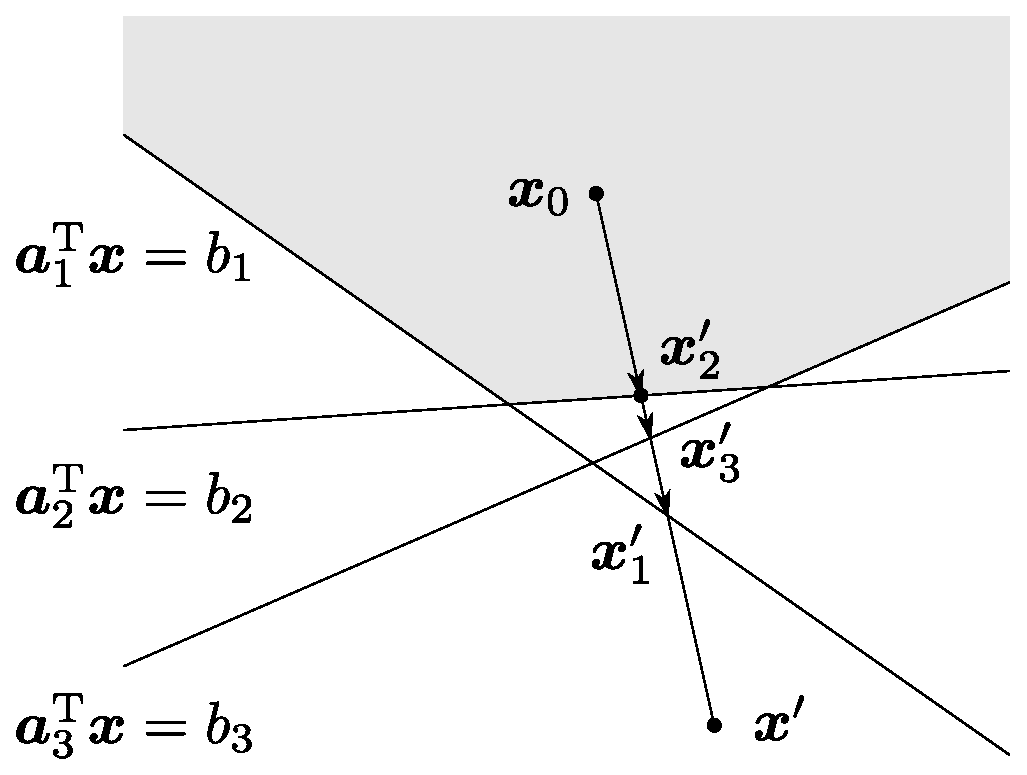
\includegraphics[width=.5\textwidth]{fig/active_set_add.eps}
\end{center}
\end{figure}

下の図のように
$\boldsymbol{x}_{0}$と$\boldsymbol{x}^{\prime}$がどちらも制約条件の境界上の点である,
すなわち$\boldsymbol{a}_{i}^{\mathrm{T}}(\boldsymbol{x}^{\prime}-\boldsymbol{x}_{0})=0$である場合は,
その境界条件を判定対象から除外すれば良いです.
\begin{figure}[h]
\begin{center}
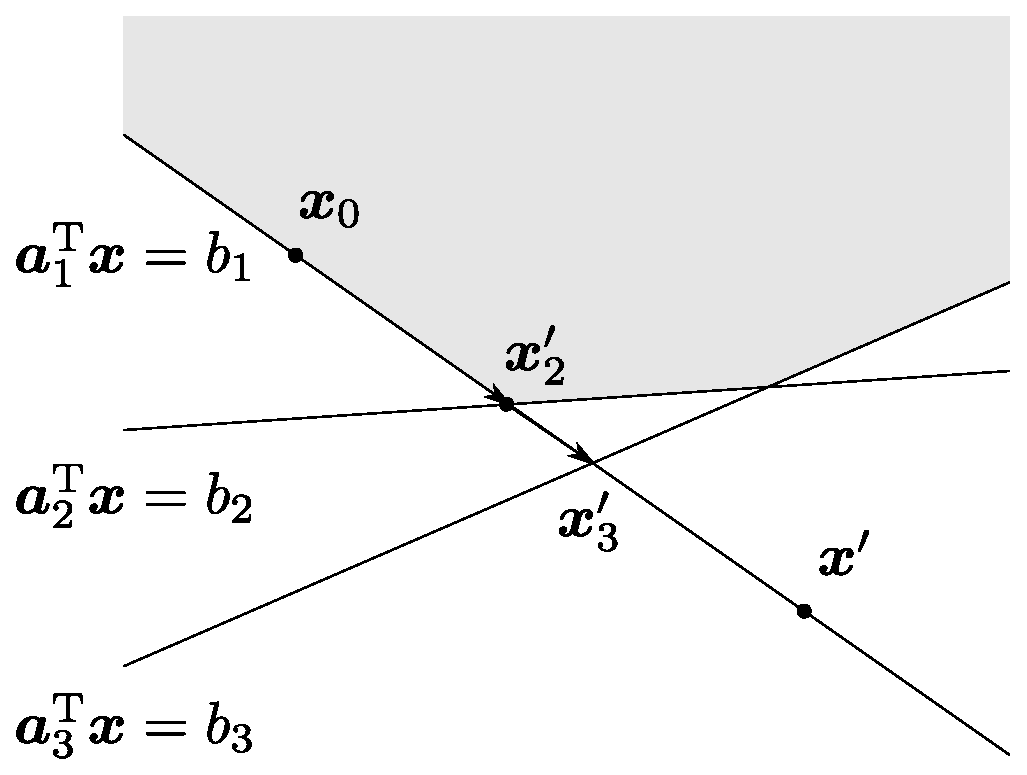
\includegraphics[width=.5\textwidth]{fig/active_set_add_deg.eps}
\end{center}
\end{figure}

以上は次の手順にまとめられます.
\begin{screen}
\begin{enumerate}
\item
$d_{\mathrm{min}}=\infty$とおく.
\item
全ての$i\in\bar{\mathcal{I}}^{\prime}$について,
 \begin{enumerate}
 \item $\boldsymbol{a}_{i}^{\mathrm{T}}\boldsymbol{x}^{\prime}\geq b_{i}$あるいは$\boldsymbol{a}_{i}^{\mathrm{T}}(\boldsymbol{x}^{\prime}-\boldsymbol{x}_{0})=0$ならばこの$i$をスキップ
 \item $d_{i}=\frac{b_{i}-\boldsymbol{a}_{i}^{\mathrm{T}}\boldsymbol{x}_{0}}{\boldsymbol{a}_{i}^{\mathrm{T}}(\boldsymbol{x}^{\prime}-\boldsymbol{x}_{0})}$とする.
 \item $d_{i}<d_{\mathrm{min}}$ならば$i_{\mathrm{min}}\leftarrow i$,$d_{\mathrm{min}}\leftarrow d_{i}$とする.
 \end{enumerate}
\item $d_{\mathrm{min}}=\infty$のままならばこの手続きを終了.
\item $\mathcal{I}^{\prime}\leftarrow\mathcal{I}^{\prime}\cup\left\{i_{\mathrm{min}}\right\}$,
$\bar{\mathcal{I}}^{\prime}\leftarrow\bar{\mathcal{I}}^{\prime}\setminus\left\{i_{\mathrm{min}}\right\}$,
$\boldsymbol{x}_{0}\leftarrow \boldsymbol{x}_{0}+d_{\mathrm{min}}(\boldsymbol{x}^{\prime}-\boldsymbol{x}_{0})$と更新する.
\end{enumerate}
\end{screen}

$\boldsymbol{x}^{\prime}$でなく$\boldsymbol{x}_{0}$を$\boldsymbol{x}_{i}^{\prime}$に置き換えることにご注意下さい.
拠り所となる$\boldsymbol{x}_{0}$は追加された有効制約を反映して更新しますが,
最適解の候補$\boldsymbol{x}^{\prime}$は新たな$\mathcal{I}^{\prime}$,$\bar{\mathcal{I}}^{\prime}$に基づいて
求め直す必要があります.


\subsection{有効制約の削除}

「$\lambda_{i}<0$($i\in\bar{\mathcal{I}}^{\prime}$)となる一つの$i$を
$\bar{\mathcal{I}}^{\prime}$から除外し$\mathcal{I}^{\prime}$に移」します.
KKT条件を考えれば,
有効制約を満たしている,すなわち$\boldsymbol{a}_{i}^{\mathrm{T}}\boldsymbol{x}^{\prime}=b_{i}$であるにもかかわらず
$\lambda_{i}<0$であるということは,
$\boldsymbol{a}_{i}^{\mathrm{T}}\boldsymbol{x}<b_{i}$の内側でさらに目的関数を減少させる$\boldsymbol{x}$が存在するということです.
それを見つけるために,
$\boldsymbol{a}_{i}^{\mathrm{T}}\boldsymbol{x}^{\prime}=b_{i}$を無効化してやる必要があります.

$\lambda_{i}$が小さいほど制約の境界$\boldsymbol{a}_{i}^{\mathrm{T}}\boldsymbol{x}^{\prime}=b_{i}$からの余裕があると期待できるので,
\begin{align*}
i^{\prime}&=\mathop{\mathrm{arg~min}}_{i}\left\{\lambda_{i}\left|i\in\mathcal{I}^{\prime}, \lambda_{i}<0\right.\right\}
\\
\mathcal{I}^{\prime}&\leftarrow\mathcal{I}^{\prime}\setminus\left\{i^{\prime}\right\}
\\
\bar{\mathcal{I}}^{\prime}&\leftarrow\bar{\mathcal{I}}^{\prime}\cup\left\{i^{\prime}\right\}
\end{align*}
とすれば良いです.
$\boldsymbol{x}^{\prime}$と一緒に$\boldsymbol{\lambda}^{\prime}$も求まっているので,
これは直接的に行えます.

\subsection{行列$\boldsymbol{Q}$の正定値性判別}

有効制約法のアルゴリズムは以上で終わりなのですが,
有効制約の追加と削除は,
冒頭に述べた$\boldsymbol{Q}$が正定値対称行列であるという仮定に依存しますので,
これが偽であった場合には正しく動作せず,
最悪の場合には無限ループに陥ります.
したがって実装上は,この仮定の真偽をチェックする処理が必須です.

行列の対称性を確認するのは容易です.
一方,行列の正定値性を確認する方法は幾つかありますが,
計算効率を考えるとCholesky分解を用いるのが最善であるように思われます.
すなわち
$\boldsymbol{Q}$が非負定値対称行列であれば,
次のようにCholesky分解することが可能です.
\begin{align*}
\boldsymbol{Q}=\boldsymbol{L}\boldsymbol{L}^{\mathrm{T}}
\end{align*}
ただし,$\boldsymbol{L}$は列フルランクな下三角行列です.
$\boldsymbol{Q}$が正定値行列であることは,
$\boldsymbol{L}$が正則であることと等価です.
よって,
$\boldsymbol{L}$が正則でない場合,あるいはそもそもこのような分解に失敗する場合は
有効制約法の適用外となり,この時点で除外できます.




\end{document}
